\documentclass[]{scrartcl}
\usepackage{Preamble}

\setcounter{section}{3}
\newcommand{\exercise}{Exercise \thesection}
\newcommand{\duedate}{2020-11-30, 23:59}

\begin{document}
\section*{\exercise}

To compile: unzip our uploaded code, and run \verb|make| inside \verb|code/|.
The slurm scripts are stored inside \verb|code/slurm/|.

\subsection{Measure Latency}
The MPI ping-pong implementation in \verb|code/src/latency.cpp| is measuring the roundtrip latency for each ping pong exchange 100000 times.
This results in the latencies observed in \autoref{fig:latency}.
Visualized in red are the times for two ranks running on the same node, while the communication between two ranks on two different nodes is visualized in blue.

\begin{figure}[ht]
    \centering
    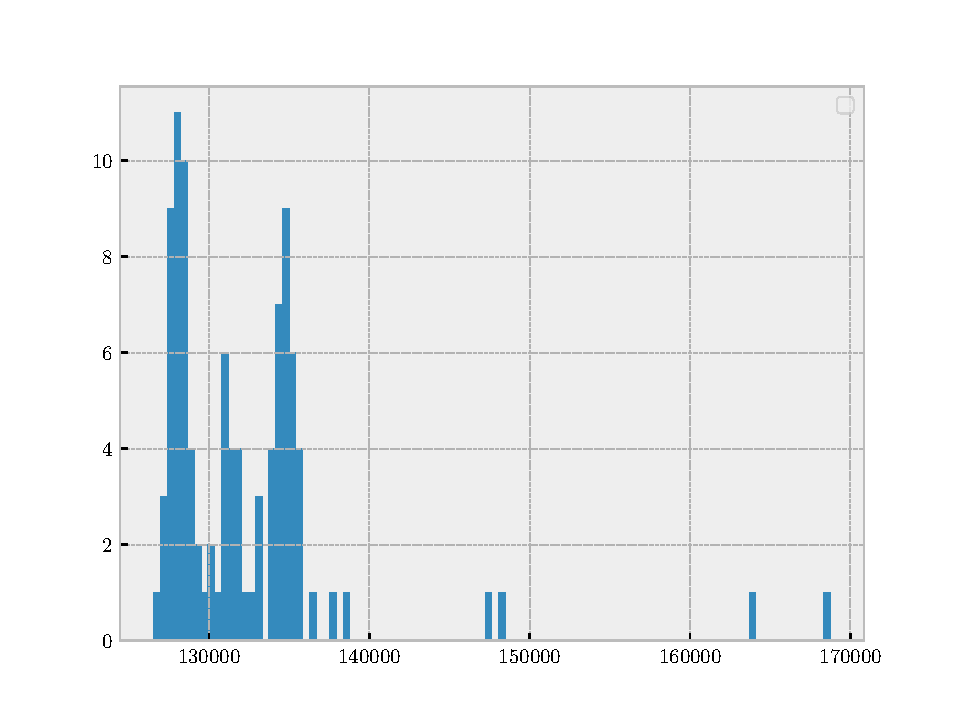
\includegraphics[width=\linewidth]{img/latency}
    \caption{Roundtrip Latency over 100000 ping-pong exchanges}%
    \label{fig:latency}
\end{figure}

Both times the Latency roughly increases linearly with message size and for the communication between nodes a distinct offset and worse latency scaling can be observed

The scaling behaves worde by two magnitudes when comparing between node-to-node and inter-node communication.

\subsection{Measure Bandwidth}
The MPI flood-test implentation in \verb|code/src/bandwidth.cpp| is measuring the bandwidth over an averarge of 1000 messages, repeating this measurement 100 times.
This results in the bandwidths observed in \autoref{fig:bandwidth}.

\begin{figure}[ht]
    \centering
    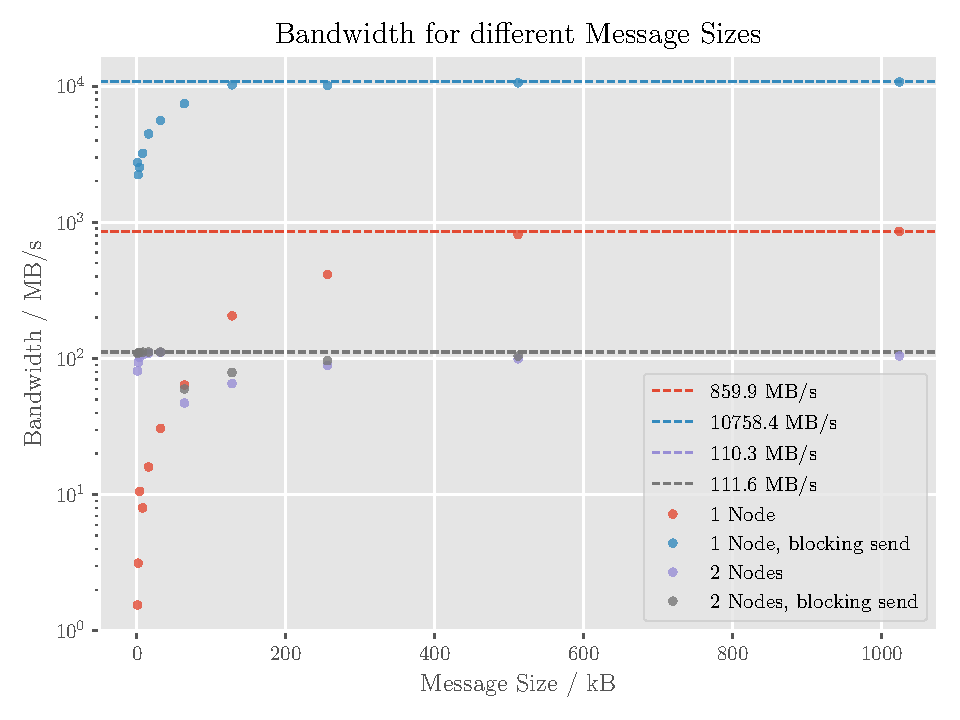
\includegraphics[width=\linewidth]{img/bandwidth}
    \caption{Bandwidth over 100000 flood-messages}%
    \label{fig:bandwidth}
\end{figure}

Here a distinct increate in bandwidth is visible when communicating betyween two nodes.
Additionally the communication between two nodes seems to be capped at $\approx$\SI{111}{MB/s}, in which case the interconnect may be the reason (\SI{1}{Gb/s} minus additional overhead additional overhead).
{\bfseries No distinct difference between blocking and non-blocking send} is observable when communication between nodes.

For the communication within one node, a distinct difference between blocking and non-blocking send was observable, here the {\bfseries blocking send bandwidth was around \SI{30}{\%} higher }.
\newpage
\subsection{Matrix multiply --- sequential}
The naïve implementation uses three nested for loops to perform the matrix multiply.
\lstset{language=C++}
\begin{lstlisting}[H]
for (size_t i = 0; i < dim; ++i) {
	for (size_t j = 0; j < dim; ++j) {
		for (size_t k = 0; k < dim; ++k) {
			C[i * dim + j] +=
			    A[i * dim + k] * B[k * dim + j];
		}
	}
}
\end{lstlisting}
On the \emph{creek} cluster a performance of \SI{0.104162}{GFLOP\per\second} is achieved.
This deviates a lot from the theoretical peak performance of the XEON E5.
There are two main problems with the implementation:
\begin{itemize}
	\item Cache utilization: The access pattern used for the naïve version
		is strided accesses to \texttt{B} are always cache misses.
	\item Hardware utilization: The processor used has 4 cores. The
		naïve Code only uses one thread.
\end{itemize}
To combat these effects the main loops were broken down into smaller blocks in order
to gain better data locality. Instead of traversing the whole matrix progress is made
block wise in each dimension. We thereby achieve both temporal and data locality, because
more values are reused (still in cache) and the stride becomes limited to cachable blocks.
The innermost loops are parallelized using \emph{OpenMP}.
\begin{lstlisting}[H]
for (size_t ii = 0; ii < dim; ii += BLOCK_SIZE) {
for (size_t jj = 0; jj < dim; jj += BLOCK_SIZE) {
for (size_t kk = 0; kk < dim; kk += BLOCK_SIZE) {
#pragma omp parallel for collapse(3)
for (size_t i = ii; i < std::min(ii + BLOCK_SIZE, dim); ++i) {
	for (size_t j = jj; j < std::min(jj + BLOCK_SIZE, dim); ++j) {
		for (size_t k = kk; k < std::min(kk + BLOCK_SIZE, dim); ++k) {
			C[i * dim + j] +=
			    A[i * dim + k] * B[k * dim + j];
		}
	}
}
}
}
}
\end{lstlisting}
Using this Code and a block size of \SI{10}{\mega B} / \SI{8}{B\per Element}
we achieve \SI{0.223383}{GFLOP/s} $\approx$ twice the performance.
This is still pretty slow! On my local machine the speedup is a lot more significant ($\approx$ factor 10).

\end{document}
